\subsection{Interacciones y alcance del sistema: Diagrama de Contexto}
A continuación mostramos el Diagrama de Contexto de la empresa. En el mismo se detallan las interacciones entre los diversos agentes de la empresa y su interacción con el sistema propuesto.

Debido a la gran cantidad de interacciones entre los agentes decidimos, por una cuestión de comprensibilidad, separar el diagrama de contexto en dos partes complementarias. Por un lado se presentan las interacciones de todos los agentes con el Sistema a implementar. Por el otro, se muestran las acciones que suceden entre los demás agentes entre si. Estos diagramas no deben ser leídos por separado, sino que son dos partes del mismo, que representa el Diagrama de Contexto final entre todos los agentes.

Además, para evitar confusiones y reducir el espacio, cada vez que se daba el caso de que había múltiples flechas de interacción entre dos agentes, la simplificamos en una sola donde listamos todas las formas en las que un agente actúa sobre el otro. Por eso, hay múltiples líneas de texto en cada flecha y estas deben ser leídas como una flecha en sí por cada línea de texto.

\begin{figure}[H]
    \centering
    \includegraphics[width=\textwidth]{imagenes/contexto-con-sistema.png}
\end{figure}

\begin{figure}[H]
    \centering
    \includegraphics[width=\textwidth]{imagenes/contexto-sin-sistema.png}
\end{figure}

\newpage

\subsection{Requerimientos del sistema: Diagrama de Objetivo}
En este diagrama detallamos como la implementación del sistema propuesto colaborará con la mejora de los procesos de la empresa.

El diagrama de objetivos se presenta con la idea de ser leído de izquierda a derecha. Frecuentemente, tratamos de colocar los objetivos que se suceden entre sí de esta forma para 'simular' los diferentes pasos que se suceden a través del tiempo.

Separamos el diagrama en varias partes (como el Diagrama de Contexto) varias veces debido al tamaño del mismo. Estos gráficos se deben leer como las diferentes partes de un mismo diagrama. Asi, presentamos primero las ramas superiores que engloban los objetivos de más alto nivel y luego mostramos como se va completando cada rama con su diagrama correspondiente.

\subsubsection{Objetivos principales}

\begin{figure}[H]
    \centering
    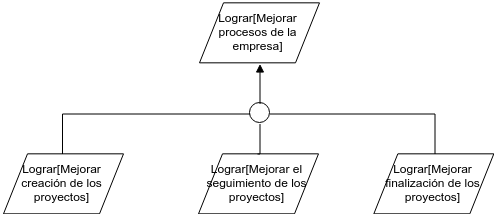
\includegraphics[width=\textwidth]{imagenes/objetivos-principales.png}
\end{figure}

En esta figura se ven los objetivos de mas alto nivel que luego detallamos en las siguientes subsecciones para cada uno de los subobjetivos que aparecen.

\subsubsection{Creacion del proyecto}

\begin{figure}[H]
    \centering
    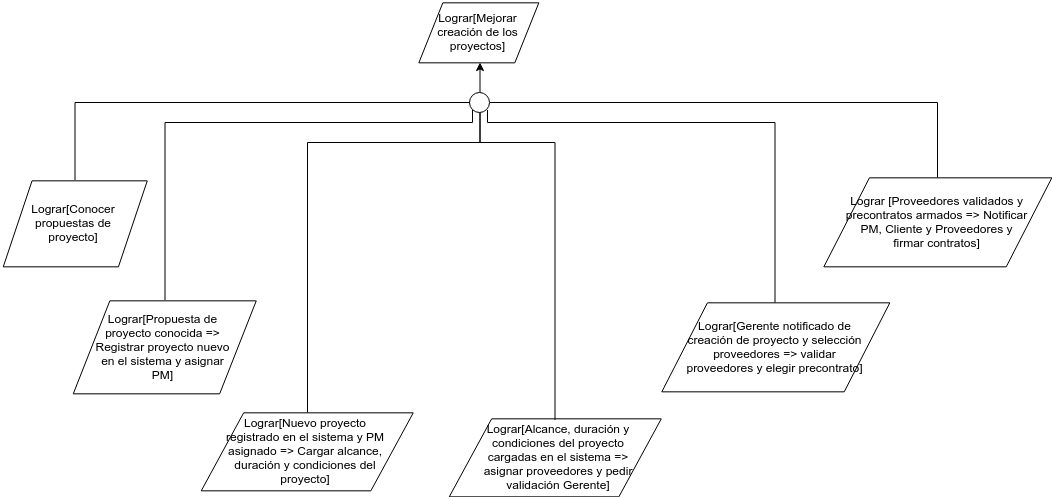
\includegraphics[width=18cm, keepaspectratio]{imagenes/objetivos-creacion-principal.png}
\end{figure}

Aca se pueden ver los objetivos primarios de Creacion de proyecto, el desgloce se muestra en los proximos graficos donde en cada figura podemos ver el detalle de cada subobjetivo con orden de aparicion de izquierda a derecha.

\vspace{1em}

\begin{figure}[H]
    \centering
    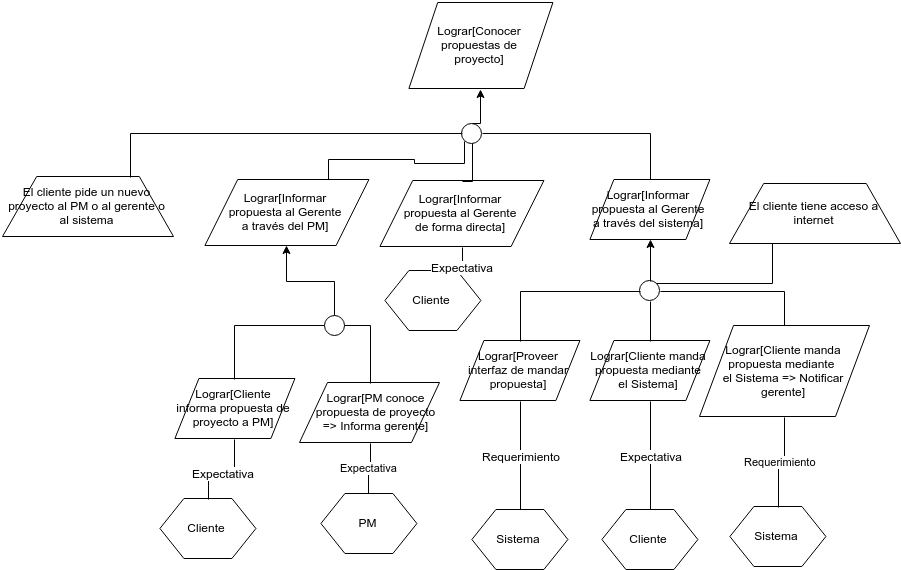
\includegraphics[width=\textwidth]{imagenes/objetivos-creacion-1.png}
\end{figure}

\vspace{1em}

\begin{figure}[H]
    \centering
    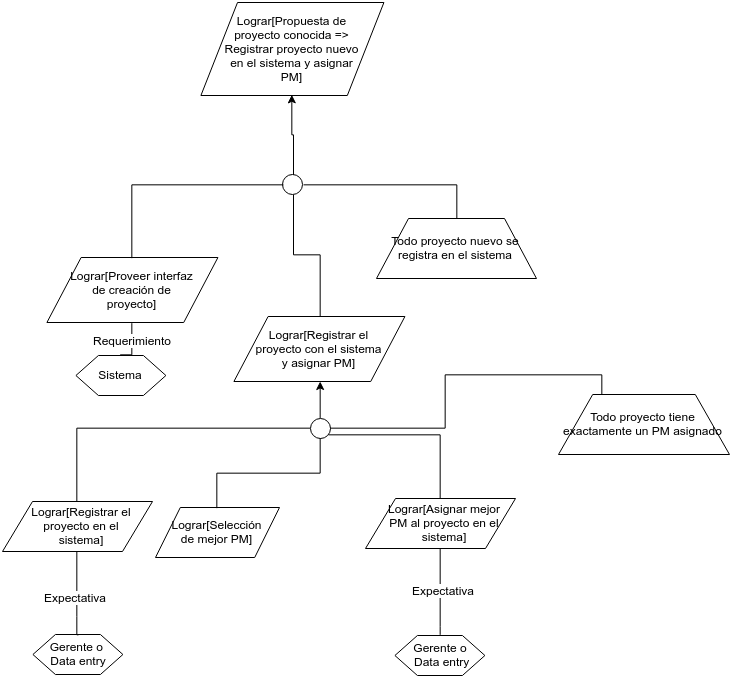
\includegraphics[width=\textwidth]{imagenes/objetivos-creacion-2.png}
\end{figure}

\subsubsection{Seleccion mejor PM}

\begin{figure}[H]
    \centering
    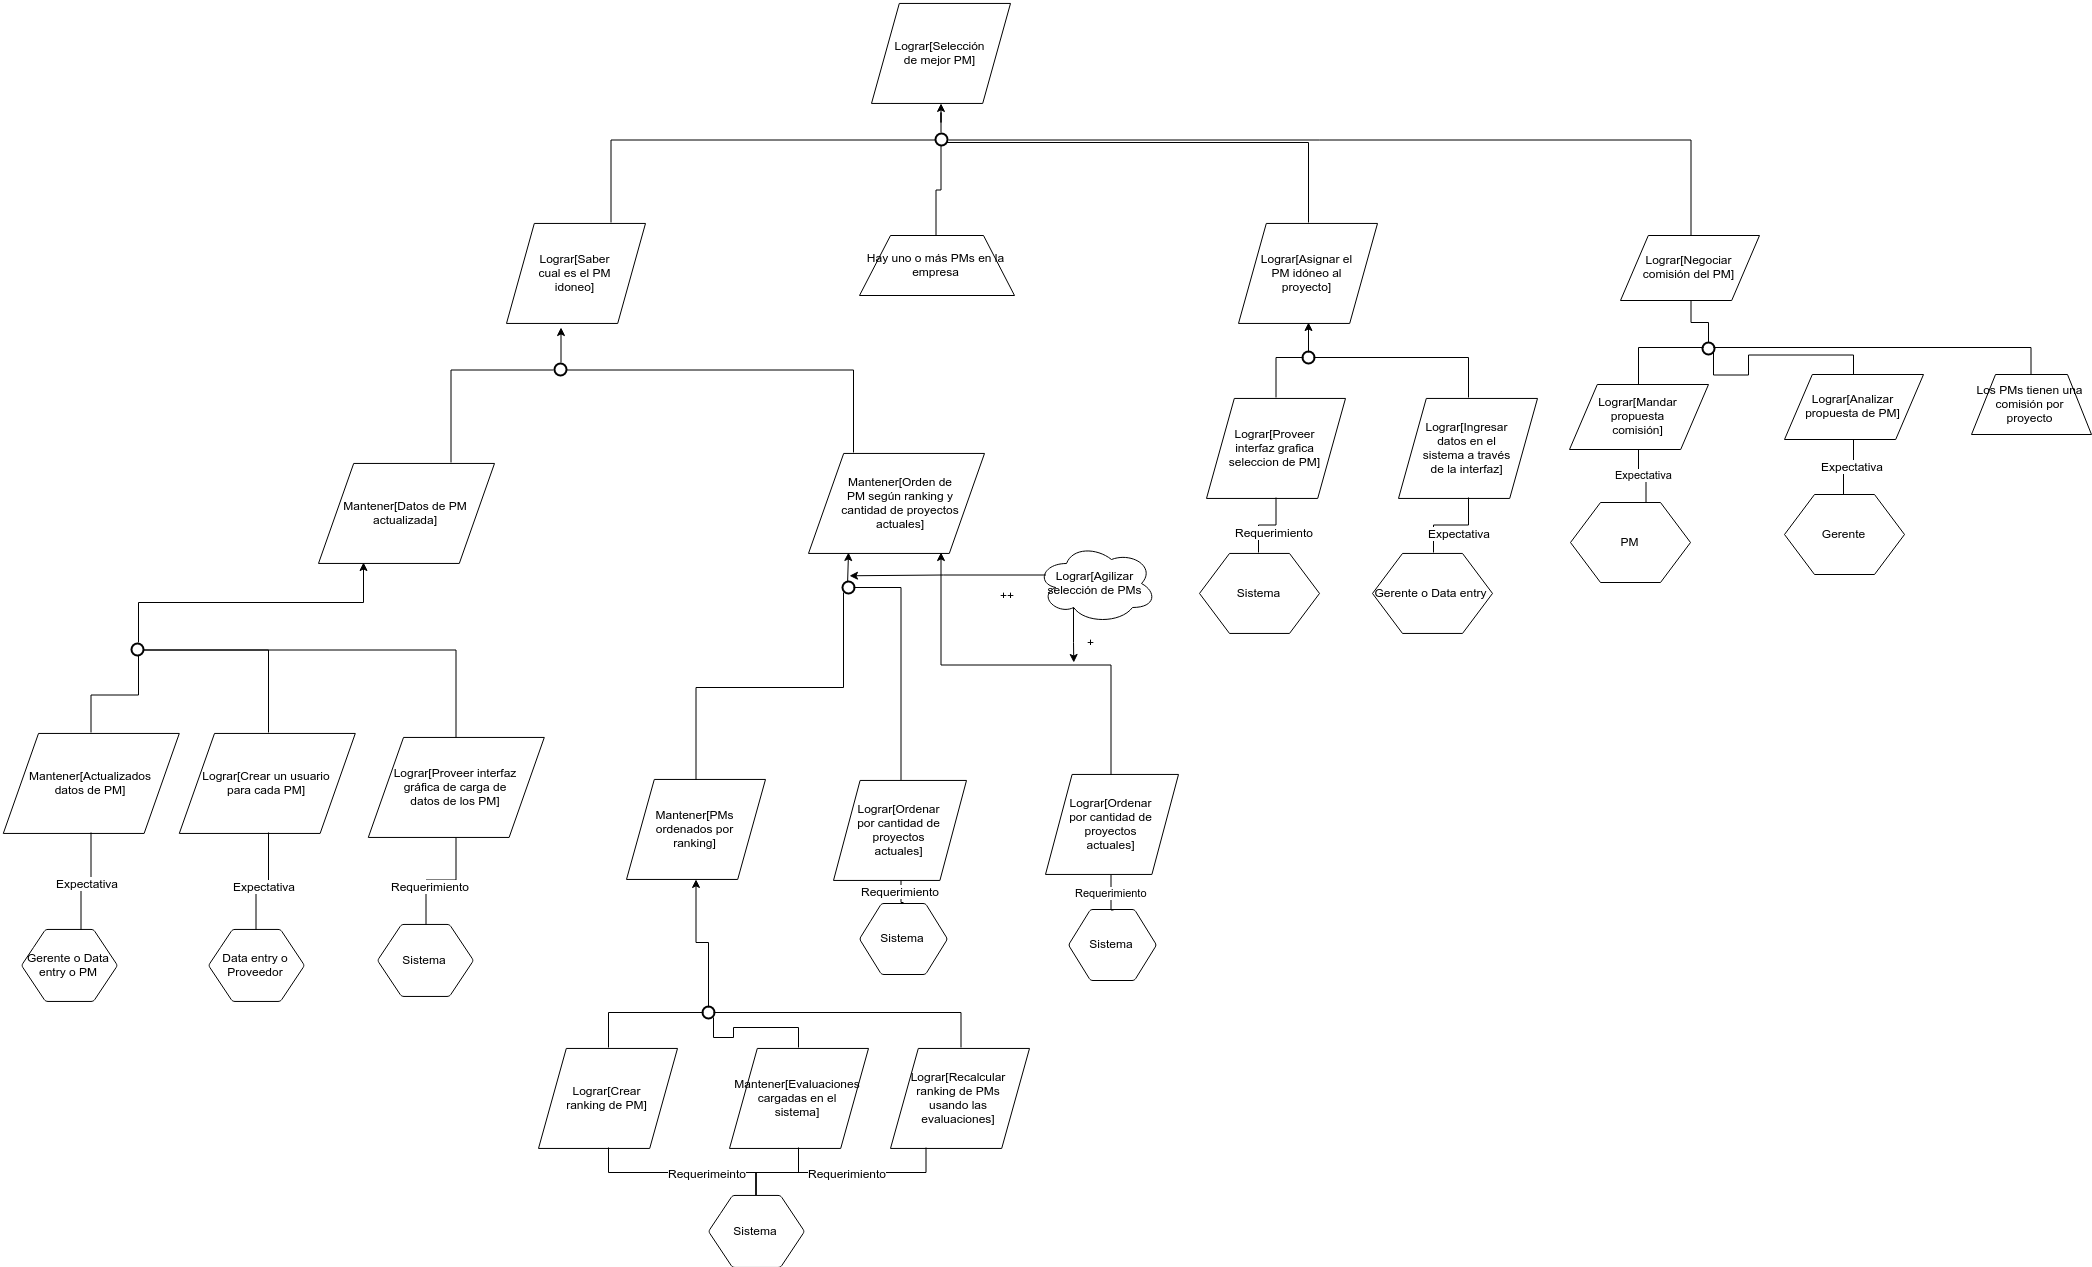
\includegraphics[width=9.5in, keepaspectratio, angle=90]{imagenes/objetivos-seleccion-mejor-pm.png}
\end{figure}

Podemos ver todos los objetivos que contribuyen a elegir el mejor PM para el proyecto dado.

\subsubsection{Seleccion mejor proveedor}

\begin{figure}[H]
    \centering
    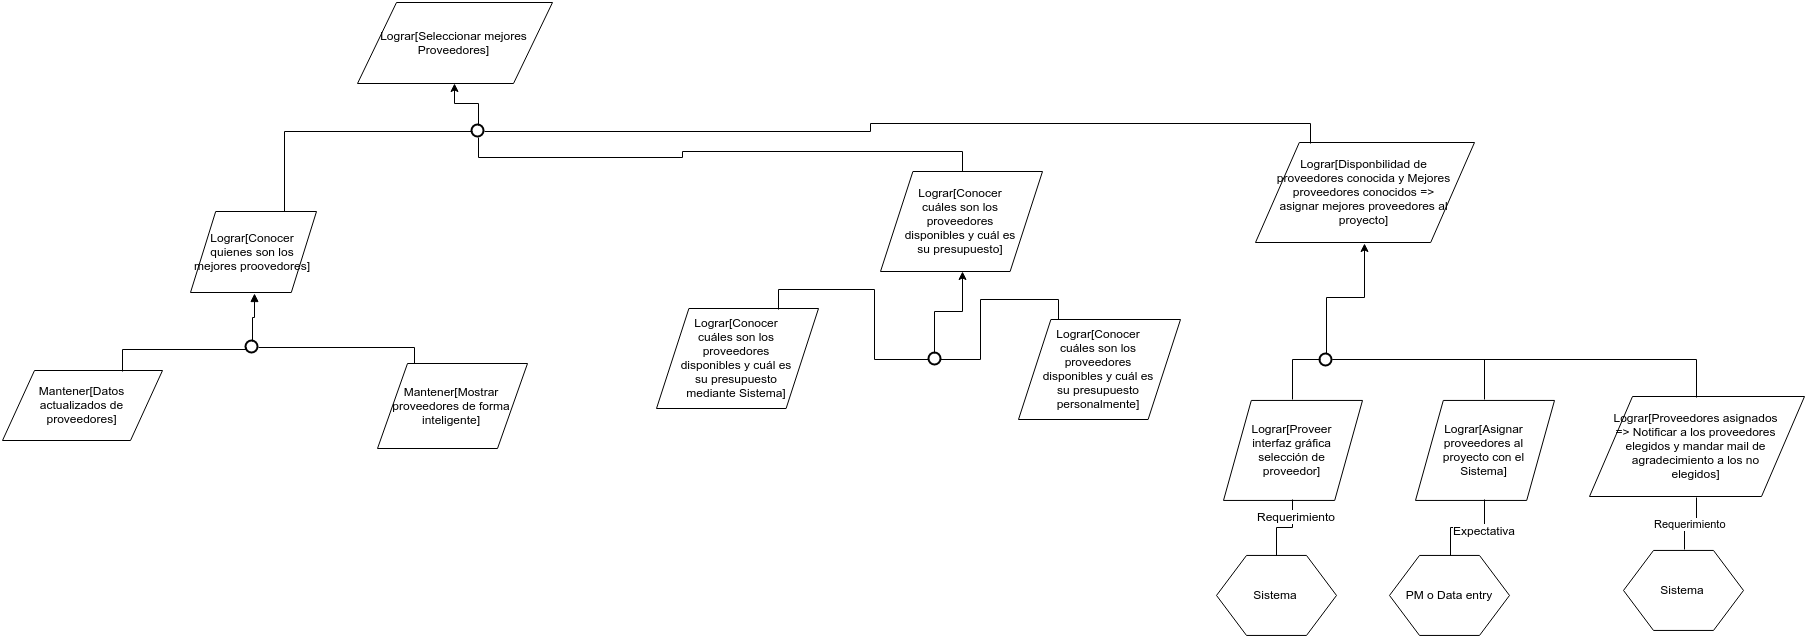
\includegraphics[width=9in, keepaspectratio, angle=90]{imagenes/objetivos-seleccion-mejor-proveedor-principal.png}
\end{figure}

Estos son los subobjetivos principales para elegir los mejores proveedores para el proyecto. El desgloce de los 4 objetivos que quedan en las figuras siguientes.

\begin{figure}[H]
    \centering
    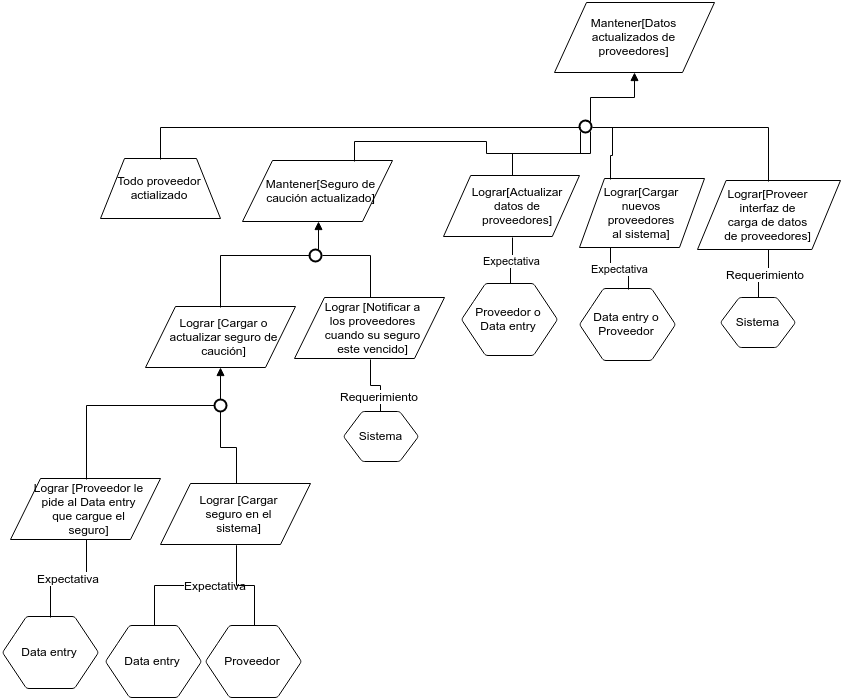
\includegraphics[width=\textwidth]{imagenes/objetivos-seleccion-mejor-proveedor-1.png}
\end{figure}

Podemos ver el primer subobjetivo de 'Lograr conocer cuales son los mejores proveedores'.

\begin{figure}[H]
    \centering
    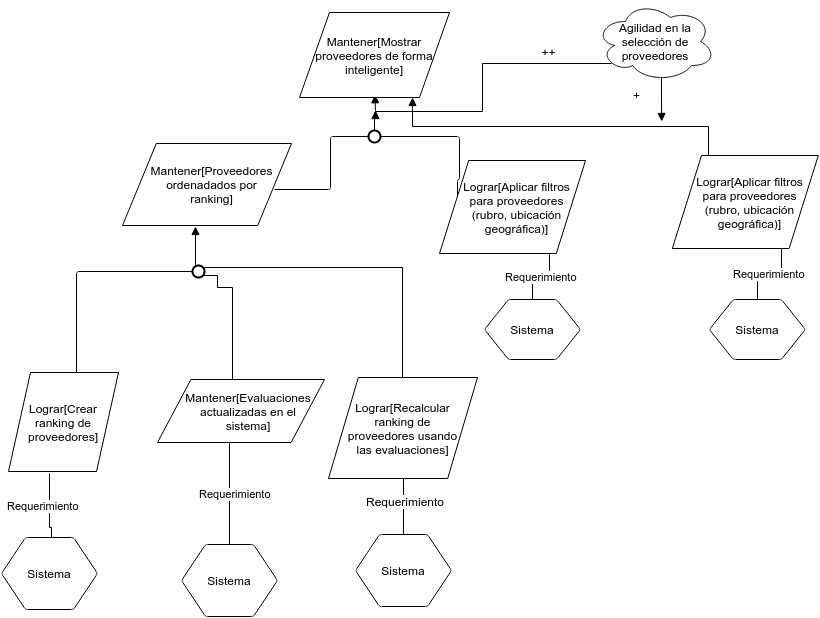
\includegraphics[width=\textwidth]{imagenes/objetivos-seleccion-mejor-proveedor-2.png}
\end{figure}

Segundo subobjetivo que contribuye a 'Lograr conocer cuales son los mejores proveedores'.

\begin{figure}[H]
    \centering
    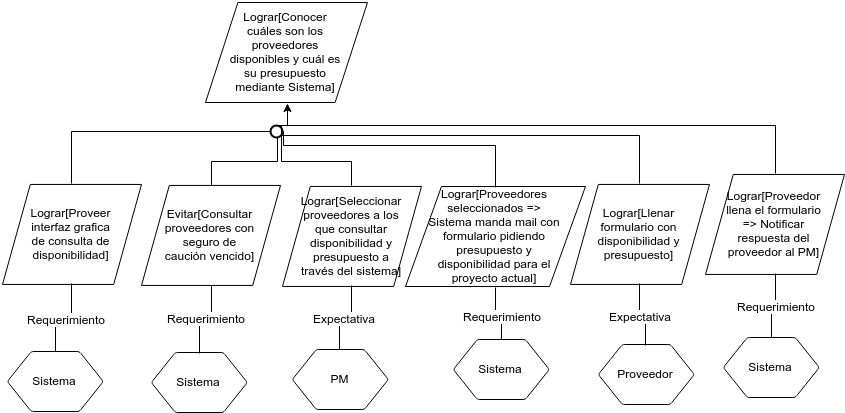
\includegraphics[width=\textwidth]{imagenes/objetivos-seleccion-mejor-proveedor-3.png}
\end{figure}

Primer subobjetivo que contribuye a 'Lograr conocer que proveedores estan disponibles y cual es su presupuesto'.

\begin{figure}[H]
    \centering
    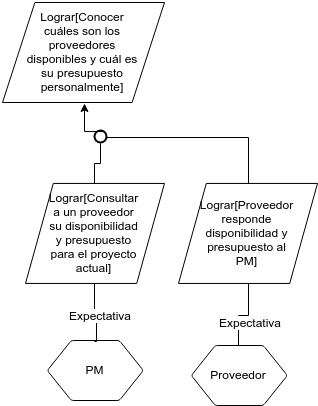
\includegraphics[width=.5\textwidth]{imagenes/objetivos-seleccion-mejor-proveedor-4.png}
\end{figure}

Segundo subobjetivo que contribuye a 'Lograr conocer que proveedores estan disponibles y cual es su presupuesto'.

\subsubsection{Seguimiento del proyecto}

\includegraphics[width=\textwidth]{imagenes/seguimiento1.png}

En este grafico se muestran los niveles mas altos de 'Seguimiento de proyecto'. Aca no se ven los refinamientos de 'Mantener estado de proyectos actualizados', que estan en las siguientes figuras.

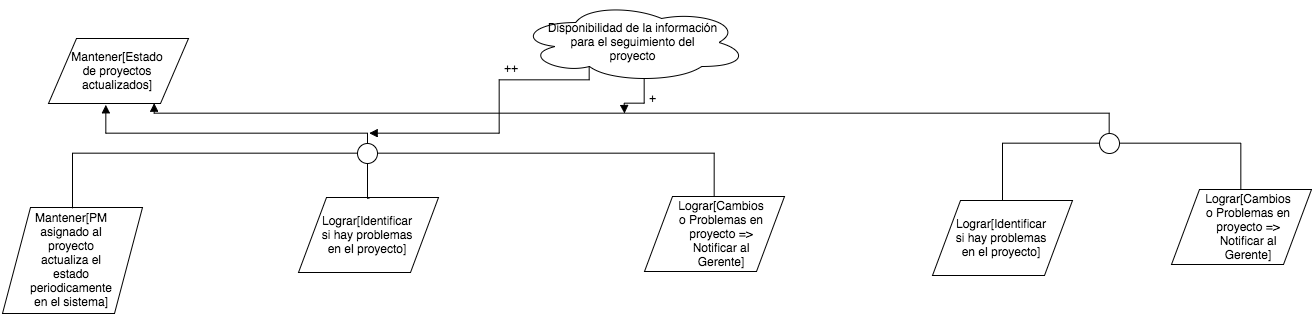
\includegraphics[width=\textwidth]{imagenes/seguimiento2.png}

En este desgloce, se puede apreciar un O-refinamiento en el cual las dos opciones tienen objetivos en comun pero uno agrega la opcion de mantener al PM actualizando obligatoriamente el estado de proyecto cada poco tiempo. Estos objetivos a su vez los desglozamos en las siguientes figuras.

\includegraphics[width=\textwidth]{imagenes/seguimiento3.png}

Aca se puede ver el Y-refinamiento de la primer alternativa.

\includegraphics[width=\textwidth]{imagenes/seguimiento4.png}

Este es el detalle de la segunda alternativa, muy similar a la primera pero con menos funcionalidad.

\newpage

\subsubsection{Finalizacion del proyecto}

\begin{figure}[H]
    \centering
    \includegraphics[width=9in, keepaspectratio, angle=90]{imagenes/objetivos-finalizacion-principal.png}
\end{figure}

Aca se pueden ver los objetivos de mas alto nivel para finalizar un proyecto. Podemos ver que hay un O-refinamiento donde se plantean dos alternativas: en una el proyecto se termina de forma 'normal' y en la otra, adicionalmente, se realizan encuestas para que el Cliente y el Gerente evaluen al PM y el PM evalue a los proveedores que participaron en el proyecto. El detalle de ellas aparece en los proximos graficos donde en cada figura podemos ver el detalle de cada subobjetivo con orden de aparicion de izquierda a derecha.

\includegraphics[width=\textwidth]{imagenes/objetivos-finalizacion1.png}

Primer subobjetivo que contribuye a la primera alternativa de 'Finalizar proyecto'.

\includegraphics[width=\textwidth]{imagenes/objetivos-finalizacion2.png}

Segundo subobjetivo que contribuye a la primera alternativa de 'Finalizar proyecto'.

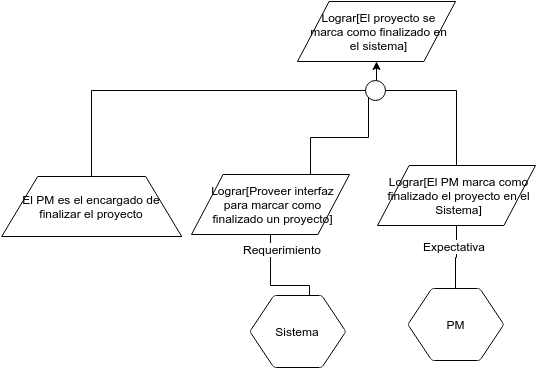
\includegraphics[width=\textwidth]{imagenes/objetivos-finalizacion3.png}

Primer subobjetivo que contribuye a la segunda alternativa de 'Finalizar proyecto'.

\includegraphics[width=\textwidth]{imagenes/objetivos-finalizacion4.png}

Segundo subobjetivo que contribuye a la segunda alternativa de 'Finalizar proyecto'.

\includegraphics[width=\textwidth]{imagenes/objetivos-finalizacion5principal.png}

Podemos ver el tercer subobjetivo que contribuye a la segunda alternativa de 'Finalizar proyecto'. A su vez, este esta dividido en tres subobjetivos que se detallan en las siguientes figuras:

\includegraphics[width=\textwidth]{imagenes/objetivos-finalizacion51.png}

Primer subobjetivo que contribuye a 'El proyecto se marca como finalizado entonces se realizan las encuestas'.

\includegraphics[width=\textwidth]{imagenes/objetivos-finalizacion52.png}

Segundo subobjetivo que contribuye a 'El proyecto se marca como finalizado entonces se realizan las encuestas'.

\includegraphics[width=\textwidth]{imagenes/objetivos-finalizacion53.png}

Tercer subobjetivo que contribuye a 'El proyecto se marca como finalizado entonces se realizan las encuestas'.
